% Created 2022-02-23 Wed 11:09
% Intended LaTeX compiler: pdflatex
\documentclass[presentation,aspectratio=169]{beamer}
\usepackage[utf8]{inputenc}
\usepackage[T1]{fontenc}
\usepackage{graphicx}
\usepackage{grffile}
\usepackage{longtable}
\usepackage{wrapfig}
\usepackage{rotating}
\usepackage[normalem]{ulem}
\usepackage{amsmath}
\usepackage{textcomp}
\usepackage{amssymb}
\usepackage{capt-of}
\usepackage{hyperref}
\usepackage{khpreamble, euscript}
\DeclareMathOperator{\atantwo}{atan2}
\newcommand*{\ctrb}{\EuScript{C}}
\newcommand*{\obsv}{\EuScript{O}}
\usetheme{default}
\author{Kjartan Halvorsen}
\date{\today}
\title{Robot móvil tipo uniciclo}
\hypersetup{
 pdfauthor={Kjartan Halvorsen},
 pdftitle={Robot móvil tipo uniciclo},
 pdfkeywords={},
 pdfsubject={},
 pdfcreator={Emacs 26.3 (Org mode 9.4.6)}, 
 pdflang={English}}
\begin{document}

\maketitle

\section{Mobile robot unicycle model}
\label{sec:org7522043}

\begin{frame}[label={sec:orgdef3f17}]{Robót móvil - modelo uniciclo}
\begin{columns}
\begin{column}{0.4\columnwidth}
\begin{center}
 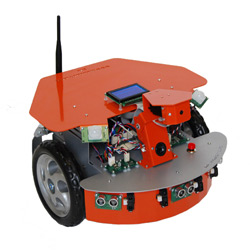
\includegraphics[width=.8\linewidth]{../figures/X80Pro.jpg}
\end{center}
\end{column}




\begin{column}{0.4\columnwidth}
\begin{center}
 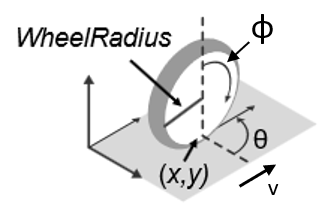
\includegraphics[width=1.0\linewidth]{../figures/unicycle_annotated.png}
\end{center}
\end{column}
\end{columns}
\end{frame}

\begin{frame}[label={sec:orgdaed7db}]{Robót móvil tipo diferencial}
\begin{columns}
\begin{column}{0.4\columnwidth}
\begin{center}
 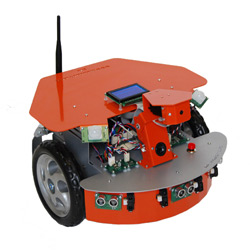
\includegraphics[width=.3\linewidth]{../figures/X80Pro.jpg}
\end{center}
\begin{center}
 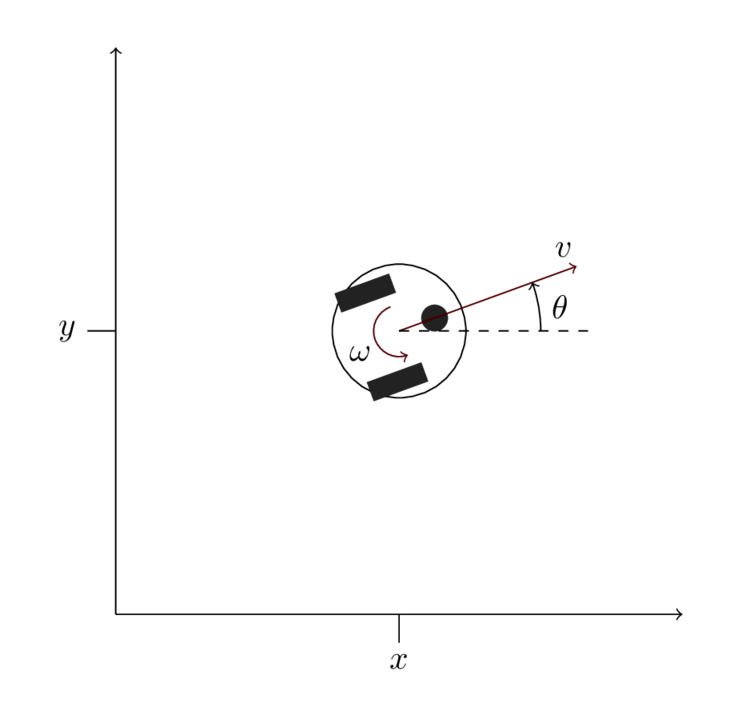
\includegraphics[width=1.0\linewidth]{../figures/unicycle-model}
\end{center}
\end{column}

\begin{column}{0.6\columnwidth}
\pause

\alert{Dinámica}

\[ \xi = \begin{bmatrix} \theta\\x\\y \end{bmatrix},   \quad u = \begin{bmatrix} \omega\\v \end{bmatrix}\]



\[\frac{d}{dt} \xi = \begin{bmatrix} \dot{\theta}\\\dot{x}\\\dot{y} \end{bmatrix} = \begin{bmatrix} \omega\\ v\cos\theta\\v\sin\theta\end{bmatrix} \]


\pause

\alert{Actividad} En simulink
\end{column}
\end{columns}
\end{frame}



\begin{frame}[label={sec:orgacc7098}]{El modelo uniciclo}
\begin{columns}
\begin{column}{0.4\columnwidth}
\begin{center}
 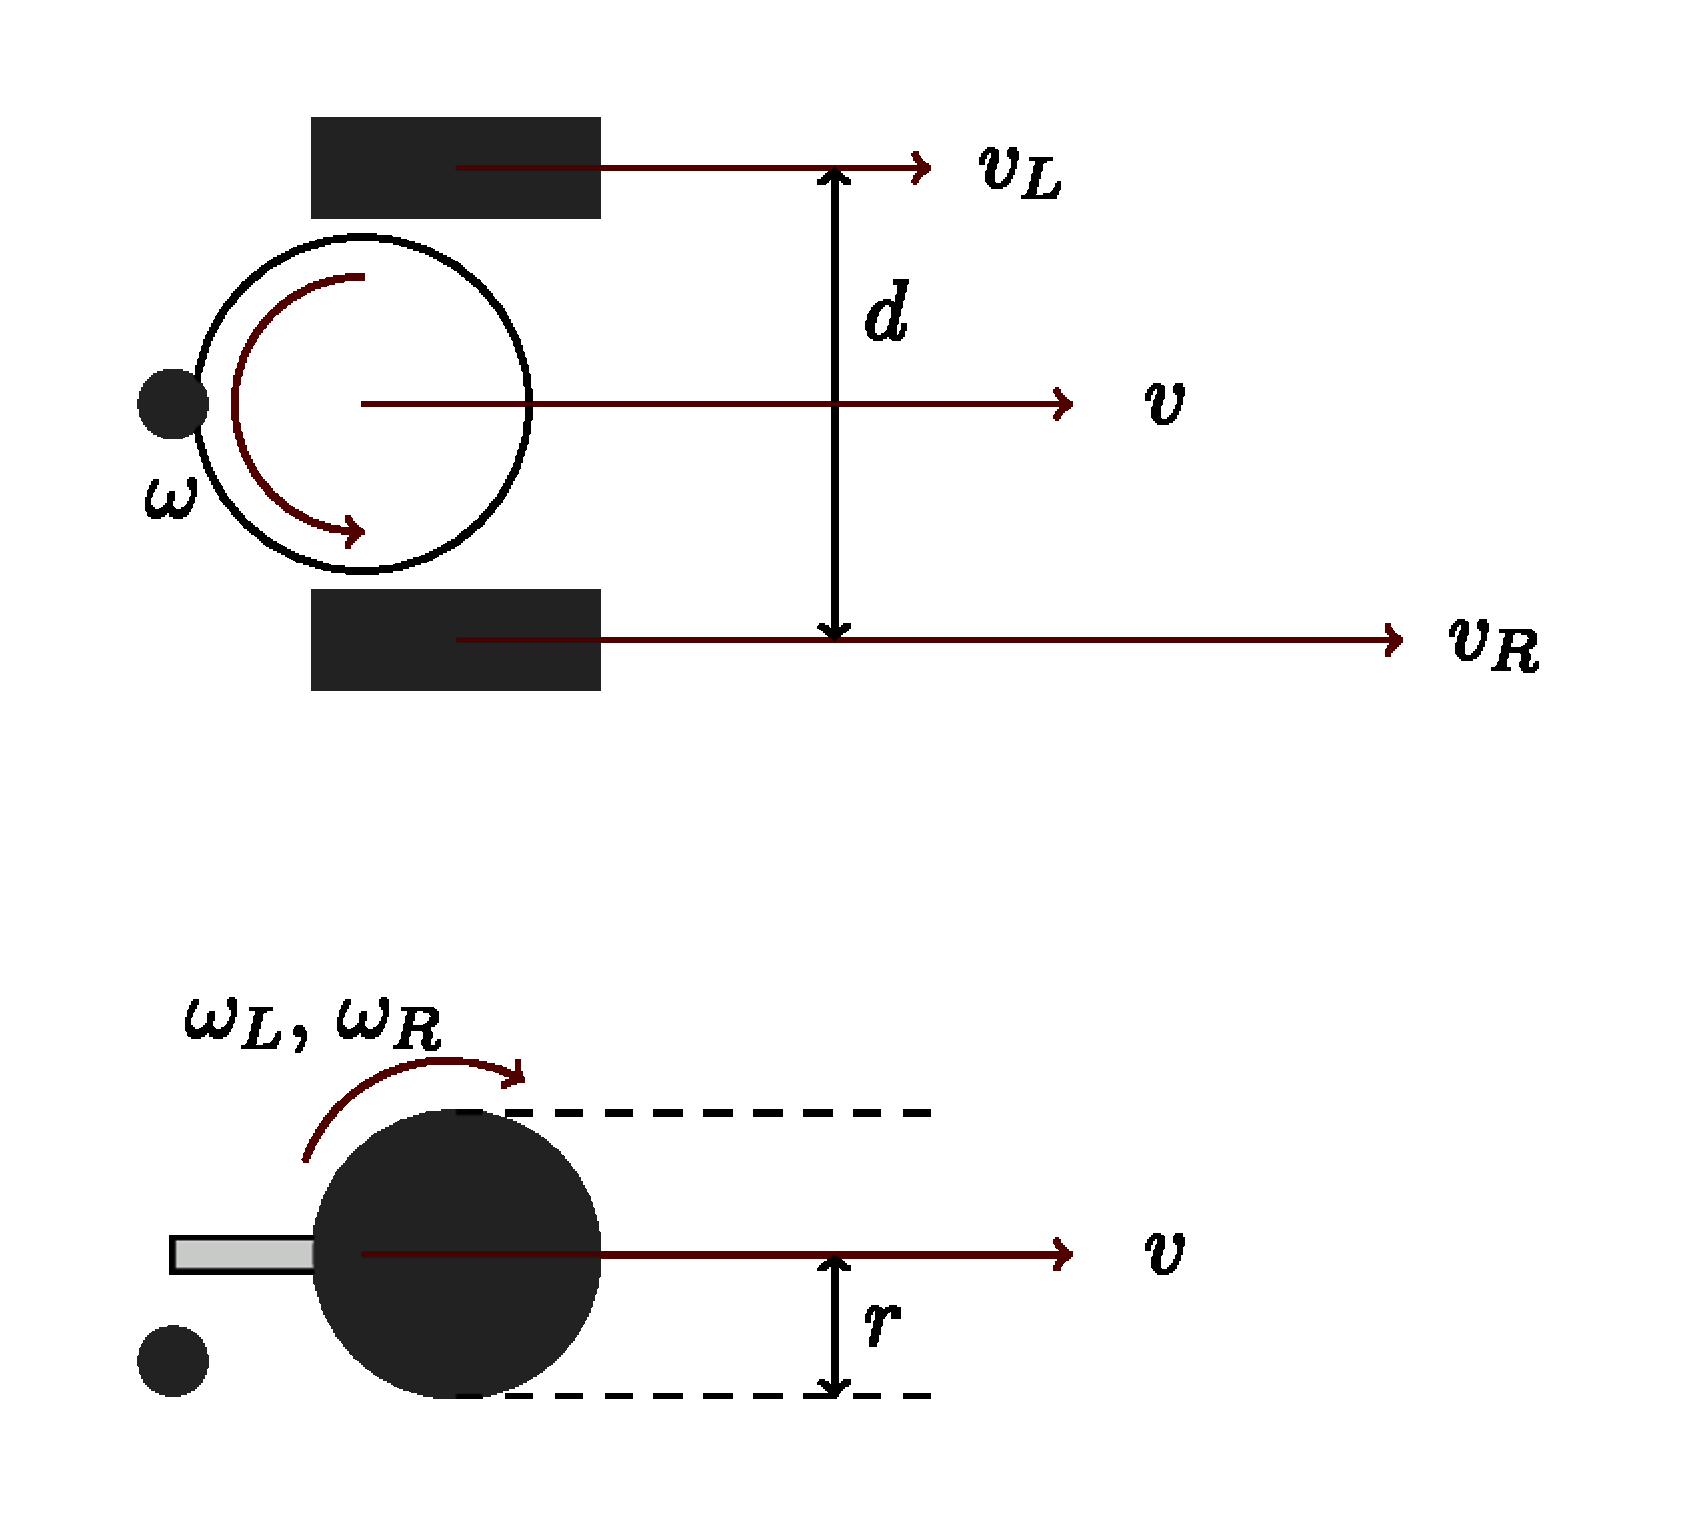
\includegraphics[width=1.0\linewidth]{../figures/unicycle-model-details}
\end{center}
\end{column}

\begin{column}{0.6\columnwidth}
\alert{Cinemática}

\pause

\alert{Actividad} Determine

\begin{enumerate}
\item La velocidad lineal (\(v_R\), \(v_L\)) de cada rueda dado su velocidad angular (\(\omega_R\), \(\omega_L\))

\item La velocidad lineal \(v\) del centro robot dado las dos velocidades \(v_R\) y \(v_L\)

\item La velocidad angular \(\omega\) del robot dado las dos velocidades \(v_R\) y \(v_L\)

\item Las relaciones invertidas. Es decir, las velocidades angulares \(\omega_R\) y \(\omega_L\) de los ruedos dado las velocidades \(v\) y \(\omega\).
\end{enumerate}
\end{column}
\end{columns}
\end{frame}


\begin{frame}[label={sec:orge03ac13}]{Implementación de la cinemática inversa}
\end{frame}

\section{Control en lazo abierto}
\label{sec:org08a6a61}

\begin{frame}[label={sec:org657d987}]{Control en lazo abierto}
\begin{columns}
\begin{column}{0.4\columnwidth}
\begin{center}
 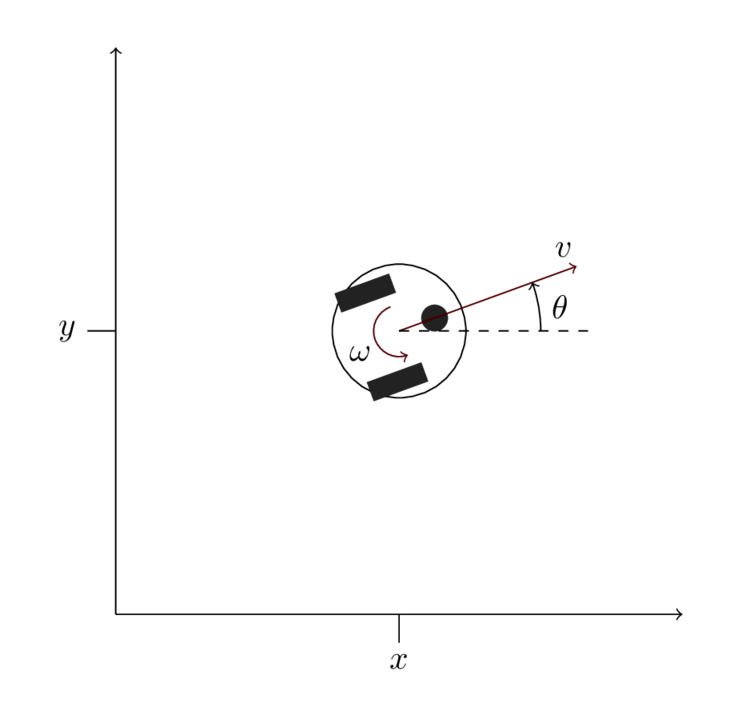
\includegraphics[width=1.0\linewidth]{../figures/unicycle-model}
\end{center}
\end{column}

\begin{column}{0.6\columnwidth}
\pause

Queremos manejar el robot de un estado inicial a otro estando. Es decir eligir una señal de entrada
$$ u(t) = \begin{bmatrix} v(t)\\\omega_t \end{bmatrix}, \; t \in [0,\, t_1) $$
que mueve el robot de una posición y orientación inicial (\(x(0)\), \(y(0)\), \(\theta(0)\)) a otra posición y orientación en \(t_1\) segundos.

\pause

\alert{Actividad}

Dibuje la señal de entrada que 
\begin{enumerate}
\item mueve el robot una distancia 1m derecho en 3 segundos.
\item cambia la dirección del robot 90 grados hacia izquierda.
\item que mueve el robot en una trayectoria de forma cuadrada con lados de 1 metros en 20 segundos.
\end{enumerate}
\end{column}
\end{columns}
\end{frame}

\begin{frame}[label={sec:org3a1ae57}]{Implementación del control en lazo abierto}
Simulink
\end{frame}
\end{document}